\documentclass[tikz,border=10pt]{standalone}
\begin{document}
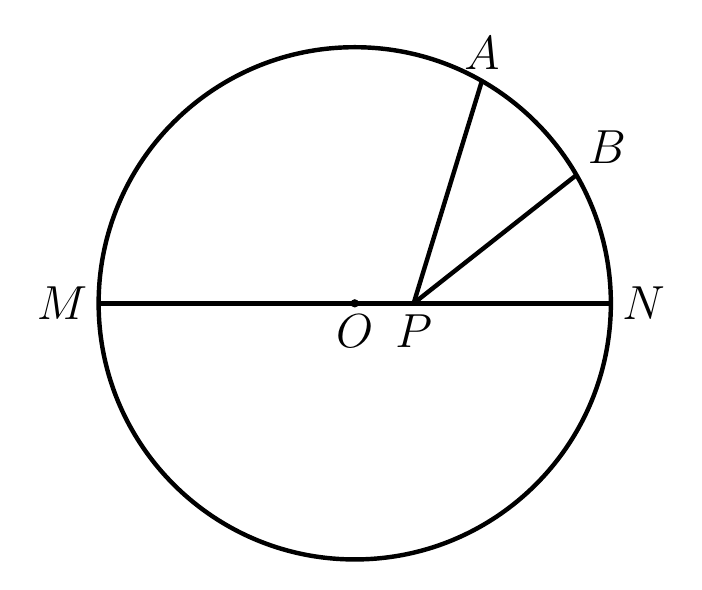
\begin{tikzpicture}[line width=1.6pt, line join=round]
% points in cm, origin at O, s = 0.020672 cm/px, y flipped
\coordinate (O) at (0,0);
\coordinate (M) at (-3.2527,0);
\coordinate (N) at (3.2527,0);
\coordinate (P) at (0.7482,0);
\coordinate (A) at (1.6146,2.8234);
\coordinate (B) at (2.8152,1.6291);

% circle (radius 157.33 px) and diameter MN
\draw (O) circle (3.2527);
\draw (M) -- (N);

% solid segments from P to A and B
\draw (P) -- (A);
\draw (P) -- (B);

% center dot at O
\fill (O) circle (1.5pt);

% labels, math mode, font from STYLE METRICS
\node[left, font=\fontsize{16.5}{19.8}\selectfont] at (M) {$M$};
\node[right, font=\fontsize{16.5}{19.8}\selectfont] at (N) {$N$};
\node[below, font=\fontsize{16.5}{19.8}\selectfont] at (O) {$O$};
\node[below, font=\fontsize{16.5}{19.8}\selectfont] at (P) {$P$};
\node[above, font=\fontsize{16.5}{19.8}\selectfont] at (A) {$A$};
\node[above right, font=\fontsize{16.5}{19.8}\selectfont] at (B) {$B$};
\end{tikzpicture}
\end{document}